\chapter{Introduction}
\label{chap:Introduction}
Since \citet{Carlowitz_1713} introduced the principle of sustainability to forestry, it plays a central role in there, and over the last centuries it has been further developed and extended. To achieve and maintain sustainability in its different specifications \citep{Speidel_1984, Schanz_1996} can be seen as one of the main goals or even the main goal of forestry. A prerequisite for such a sustainable forestry is information on the forest resources, their conditions and changes. This information is usually gained through forest inventories.

\begin{figure}
\center
  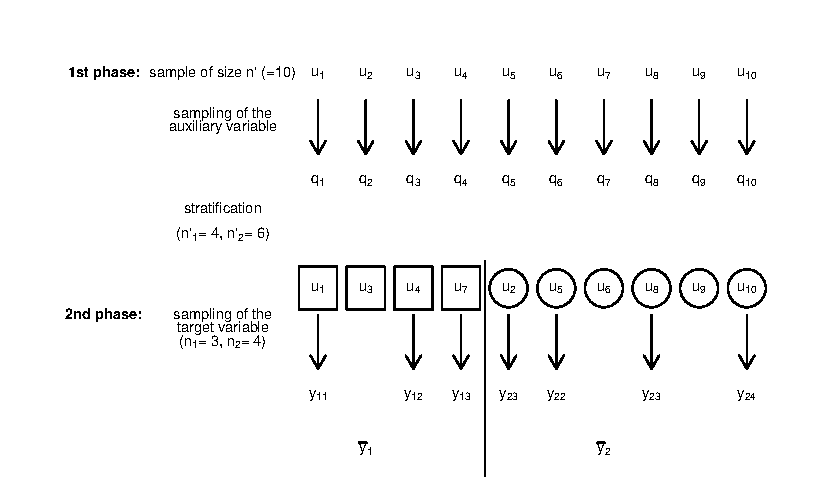
\includegraphics[width=\textwidth]{Grafiken/Introduction/example.pdf}
\caption{Example Figure.}
\label{fig:Introduction:Floatchart_2st}
\end{figure}

Reference example to \textbf{chapter \ref{chap:hzb}}.
